\section{Introduction}

\marginnote{Intended Learning Outcomes}The aim of this exercise is to introduce you to Engineering Design Process Models, Principles of Design \& Manufacture, and Project Management techniques. 
The lectures provides a overview of the techniques that are typically employed whilst the exercise provides an opportunity to put some of these techniques into practice as you design a product to meet a design brief, which you will then manufacture in your 2nd year.

Over the next five weeks you will be introduced to:

\begin{itemize}
  \item Defining Engineering Design;
  \item Design Process Models;
  \item The Design Brief and Product Design Specification;
  \item Concept Design;
  \item Concept Selection;
  \item Design for X;
  \item Rapid Prototyping; and,
  \item Project Management Essentials.
\end{itemize}

\marginnote{Support} To support the exercise, there are lectures and tutorial classes that you should attend. 
In addition, there is a Moodle course page containing support material and a Q\&A forum. 
All out of lecture and tutorial hour queries should be submitted to the Q\&A. 
This enables us to provide fair and balanced feedback across the all the groups.

As the coursework builds on the previous weeks work, it is crucial that you keep up-to-date to avoid overloading yourselves at the end. These exercises have been developed so that you can begin to experience and learn how best to manage your team and the tasks that need to be completed.

\cref{tbl-lectures} provides an overview of the lecture and pre-work that should be performed ahead of the tutorial session so you can ask for feedback in the sessions.

\begin{table}[h!]
  \caption{Supporting lecture and tutorial sessions}
  \label{tbl-lectures}
  \small
  \centering
  \footnotesize
  \begin{tabular}{c p{0.4\textwidth} p{0.4\textwidth}}
      \toprule
      
      Week & Lecture & Activities \\
      
      \midrule

      07 & 
      Exercise, Design Process Models \& Product Design Specification & 
      PDS \& Morphological Chart \\
      
      08 & 
      Concept Generation \& Concept Selection 
      & Concept Selection \\
      
      09 & 
      Embodiment Design \& Design for Assembly & 
      Embodiment Design \& Design for Assembly \\
      
      10 & 
      Design for Manufacture & 
      Design for Manufacture \\
      
      11 & 
      Project Management Essentials & 
      Design Report \\

  \bottomrule
  \end{tabular}
\end{table}


As with your Engineering Drawing classes\marginnote{Feedback}, you will be given formative feedback throughout your tutorials. These are supported by staff and post-graduate researchers. This is your opportunity to get feedback on your design work, so use this time wisely. You are expected to work outside of these hours and that you come to the tutorial sessions ready with questions concerning your design.

\marginnote{Significance of Engineering Design}Engineering Design is the discipline of transferring your theoretical knowledge and understanding of engineering systems into practical and usable products. You may find it interesting to discover that up to 80\% of the committed cost of a product occurs when decisions are made early-on in its design (\cref{fig-committed}).\cite{ullman2002}\cite{corbett1986}\cite{mileham1993}

\begin{figure}[t!]
  \centering
  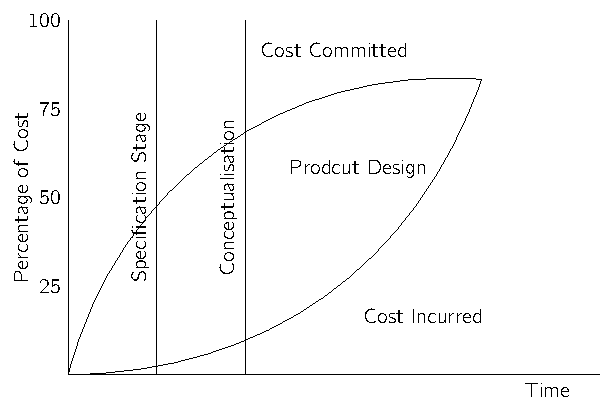
\includegraphics[width=0.9\textwidth]{figs/committed-cost.pdf}
  \caption[The committed cost during a design project]{The committed cost during a design project~\citep{ullman2002}}
  \label{fig-committed}
\end{figure}

It is the objective of the designer to consider all the potential implications of these decisions and their impact across the Product's Lifecycle. This is becoming evermore critical as companies become more reliant on the sale of products as part of a service, which is often referred to as Product Service Systems. For example, Rolls-Royce's sale strategy is now focused on the idea of `Power by the Hour'. Thus, issues in the design of the product can greatly impact the profitability and safety of the service they provide.

With companies becoming ever-more global, engineering teams are often collaborating across the world on new product development. The competencies and skills that you will develop throughout your design exercises in Bath will enable you to meet these challenges head-on.

\marginnote{Thirty-Three Percent}It may also be interesting to know that the majority of you will progress into higher-levels of management, be it in an engineering, consultancy, medical, banking, start-up and/or other industrial sectors. The success of engineers in business is further demonstrated by the fact that a third of the top Chief Executive Officers (CEO's) have an engineering degree.\cite{bi2011}\cite{hbr2014} Nearly as many who have an MBA! 
